\section{Sistemi di tipo}
\label{sec:3-type-systems}

Durante la genesi di ogni linguaggio di programmazione, una delle scelte più significative riguarda
l'introduzione di un sistema per gestire i tipi di variabili ed espressioni.

\noindent Tali sistemi di tipo sono di fatto insiemi di regole logiche che permettono
di assegnare una proprietà \textit{"tipo"} a ciascuno dei termini del linguaggio che ne necessitano.

\noindent Sono principalmente suddivisi in due categorie:
\begin{itemize}
    \item \textbf{tipizzazione statica}: i tipi sono definiti a tempo di compilazione
          e non possono cambiare mentre il programma è in esecuzione;
    \item \textbf{tipizzazione dinamica}: i tipi vengono stabiliti durante l'esecuzione
          e possono cambiare in qualsiasi momento.
\end{itemize}

\noindent Oltre a questa distinzione esistono varie sfumature e approcci differenti,
informalmente classificati in base alla rigidità delle regole di tipizzazione.
Si parla di \textit{tipizzazione debole} quando ad esempio sono consentite conversioni implicite tra tipi diversi,
\textit{tipizzazione forte} se sono impedite, oppure qualora sia o meno disponibile l'aritmetica dei puntatori.

\newpage

\begin{figure}[H]
    \centering
    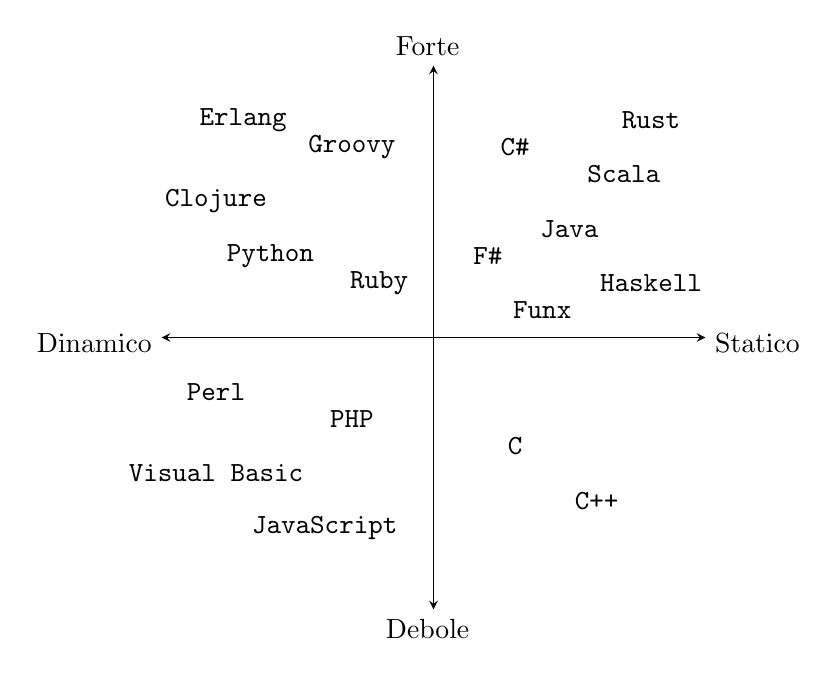
\begin{tikzpicture}
        \begin{axis}[
                % axis shenanigans
                width=0.7\textwidth, height=0.7\textwidth,
                xmin=-10, xmax=10,
                ymin=-10, ymax=10,
                xtick={-10},
                extra x ticks={10},
                ytick={-10},
                extra y ticks={10},
                % multiple labels for axes are actually tick labels
                xticklabels={Dinamico},
                extra x tick labels={Statico},
                yticklabels={Debole},
                extra y tick labels={Forte},
                % mess of a latex, with inconsistent package syntax
                tick style={draw=none},
                x tick label style={left},
                extra x tick style={xticklabel style={right}},
                y tick label style={below},
                extra y tick style={yticklabel style={above}},
                axis lines=middle,
                axis line style={stealth-stealth},
                clip=false
            ]
            % bleh
            \node at (axis cs:-8,-5) {\texttt{Visual Basic}};
            \node at (axis cs:-4,-7) {\texttt{JavaScript}};
            \node at (axis cs:-8,-2) {\texttt{Perl}};
            \node at (axis cs:-3,-3) {\texttt{PHP}};
            % meh
            \node at (axis cs:-7,8) {\texttt{Erlang}};
            \node at (axis cs:-8,5) {\texttt{Clojure}};
            \node at (axis cs:-3,7) {\texttt{Groovy}};
            \node at (axis cs:-6,3) {\texttt{Python}};
            \node at (axis cs:-2,2) {\texttt{Ruby}};
            % okay
            \node at (axis cs:3,-4) {\texttt{C}};
            \node at (axis cs:6,-6) {\texttt{C++}};
            % good
            \node at (axis cs:3,7) {\texttt{C\#}};
            \node at (axis cs:4,1) {\texttt{Funx}}; % bleh amongst the good
            \node at (axis cs:5,4) {\texttt{Java}};
            \node at (axis cs:2,3) {\texttt{F\#}};
            \node at (axis cs:7,6) {\texttt{Scala}};
            \node at (axis cs:8,2) {\texttt{Haskell}}; % hell yeah
            \node at (axis cs:8,8) {\texttt{Rust}}; % divine
        \end{axis}
    \end{tikzpicture}
    \caption{Alcuni linguaggi e loro sistemi di tipo}
    \label{fig:3-languages-type-systems}
    \vspace{8mm}
\end{figure}

\noindent Grazie ai tipi dinamici, linguaggi quali \texttt{Python} e \texttt{JavaScript} permettono
veloce prototipazione, flessibilità e codice più conciso, a discapito però di una più alta
probabilità di incontrare errori importanti a runtime, piuttosto che in fase di compilazione.


Al contrario, i tipi statici spesso migliorano naturalmente la mantenibilità di un progetto:
viene limitata la possibilità di scorciatoie nello sviluppo, ma si hanno maggiori garanzie di correttezza,
in quanto il compilatore può implementare ulteriori controlli e segnalare errori semantici più precisi già
prima dell'esecuzione del programma.

\noindent D'altro canto, l'obbligo di specificare i tipi di ogni variabile, oggetto, funzione e
parametro può risultare tedioso e talvolta ridondante; molti linguaggi moderni,
tra cui \texttt{Haskell} e \texttt{Rust}, ovviano magistralmente a quest'inconvenienza tramite
l'uso dell'inferenza di tipo.

\noindent Gli algoritmi di inferenza introducono numerosi benefici, in particolare:
\begin{itemize}
    \item la scrittura del codice è meno onerosa per lo sviluppatore a prescindere dal sistema di tipi utilizzato,
          e diviene quindi estremamente vantaggioso utilizzare tipi statici;
    \item le annotazioni ora opzionali possono essere aggiunte dal programmatore quando vi sono casi difficili
          da disambiguare automaticamente, oppure per migliorare la leggibilità del codice;
    \item gli strumenti di sviluppo per il linguaggio possono sfruttare informazioni fornite dal motore di inferenza
          per suggerire il tipo delle espressioni e arricchire i messaggi di errore e di warning.
\end{itemize}